% EN48 c07 | 原书 p.91 中部–110 上部（PDF 100–119） | 第 4 章 §4.2–4.3
% 块边界：p.91 上半属 §4.1 证明收尾（归 c06）；p.110 下半起为 §4.4（归 c08）。
\subsection{定义 $H^0(\mathrm{FS}(Y,v_0))$ 的背景}

% ===== 原书 p.91 =====

以下背景取自 [Sei08]。

% ===== 原书 p.92 =====

\begin{figure}[htbp]
\centering
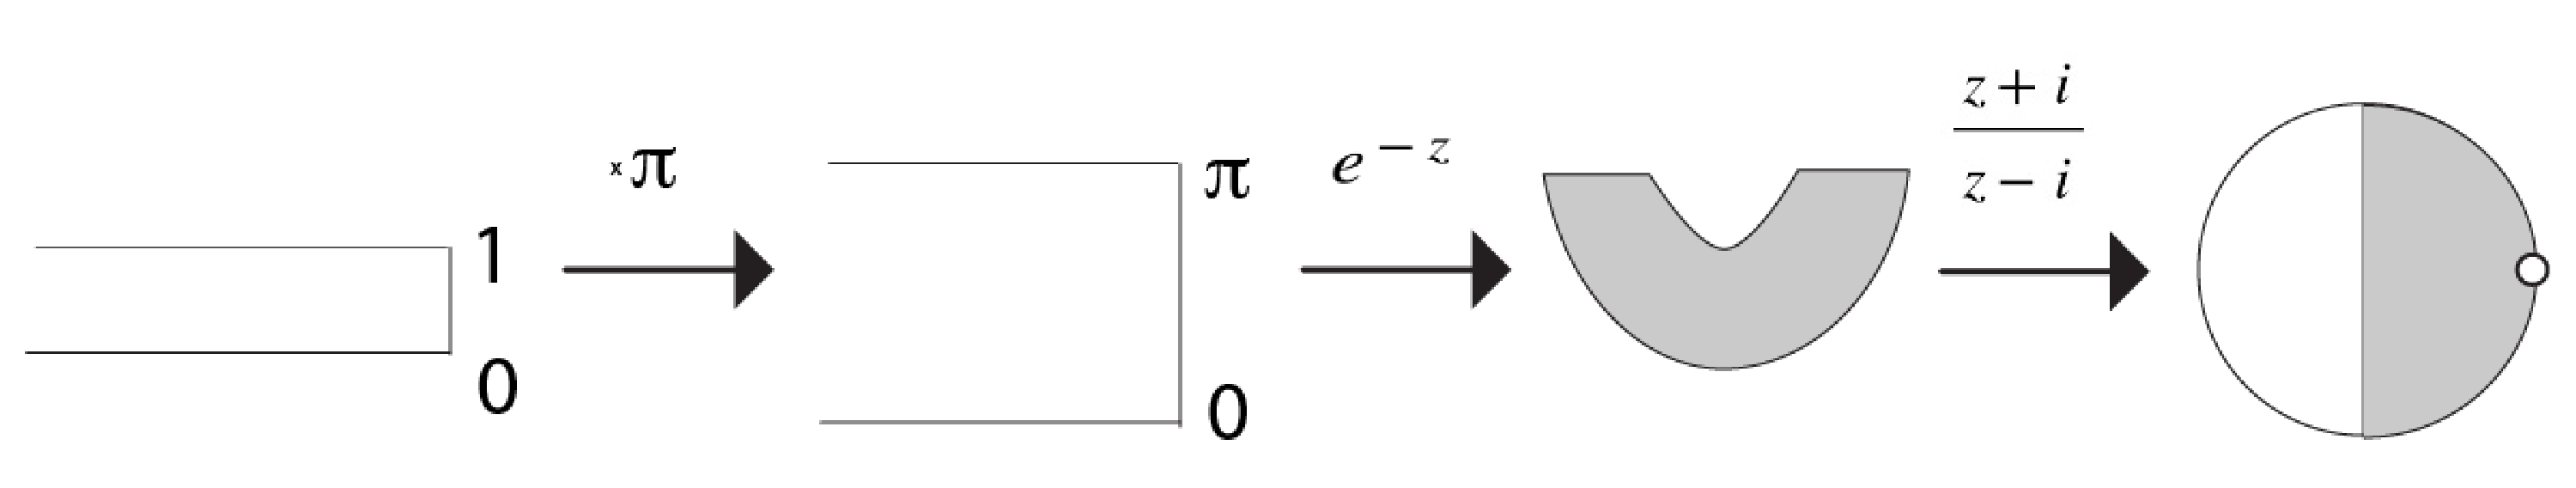
\includegraphics[width=0.8\textwidth]{figures/fig_4_2.png}
\caption{条状端的例子（原书 p.92）}
\label{c7:fig-strip-end}
\end{figure}

\begin{remark}[记号]\label{c7:rem-notation}
我们从辛纤维丛 $v_0\colon Y\to\C$ 讲起。它不是正合的，因为纤维是紧环面。
$Y$ 本身没有边界；不过下文会限制到原点附近的一个小圆盘，那里有边界。
按 [Sei08] 的术语，纤维是环面，所以没有水平边界；但取底空间中一个紧邻域的原像，就得到竖直边界。

我们考虑的近复结构满足两条：1）与上面定义的 $\omega$ 相容；2）在边界附近等于由复环面坐标诱导的标准结构 $J_0$。
这个集合记作 $\cJ_{\mathrm{reg}}(Y,\partial Y)$。它非空，因为含 $J_0$；它又可缩，论证与「全体 $\omega$-相容近复结构之集可缩」相同。
\end{remark}

\transnote{「水平边界 / 竖直边界」是 [Sei08] 的术语：水平边界指纤维方向的边界，竖直边界指底空间方向的边界。这里纤维是闭环面，没有水平边界；把底空间截成圆盘，才出现竖直边界。后文说「边界附近取 $J_0$」，指的是这个竖直边界。}

\begin{definition}[区域]\label{c7:def-domains}
带 puncture 的边界黎曼面 $S$，指这样一组数据：一个紧、连通、带边且边界非空的黎曼面，在其边界上挖去若干 puncture；再给 $\partial S$ 的每个连通分支指定一个正合拉格朗日。

我们再给 $S$ 加一层额外结构，称为「刚性化」。把 puncture 分为「正」「负」两类，并分别用嵌入
\[
\eps\colon(-\infty,0]_s\times[0,1]_t\to D,
\qquad
\eps\colon[0,\infty)_s\times[0,1]_t\to D
\]
定义负、正 puncture $\zeta^\pm$ 处的条状端，要求 $\lim_{s\to\pm\infty}\eps(s,t)=\zeta^\pm$。
这样的 $S$ 叫作带条状端的黎曼面。
\end{definition}

\begin{example}\label{c7:ex-strip-end}
本文中 $S$ 只会是三种情形之一：单位圆盘 $D$；两个圆盘沿边界上一点粘起来；一个圆盘与一族球之并。每种情形都可能带若干 puncture。

后文用来粘接两个圆盘的一个条状端是
\[
(-\infty,0]\times[0,1]\ni(s,t)
\mapsto
\eps_-(s,t):=\frac{e^{-\pi(s+it)}+i}{e^{-\pi(s+it)}-i}
=\frac{z+i}{z-i}\circ e^{-z}\circ\pi\cdot(s+it)\in D\setminus\{1\}.
\]
注意 $-\infty$ 就是该 puncture，它在圆盘中映到 $\zeta^-:=1$。见图~\ref{c7:fig-strip-end}。
\end{example}

\transnote{公式里的复合次序由图~\ref{c7:fig-strip-end} 读出：条带先经 $\pi$ 变成一条宽度为 $\pi$ 的方块，再经 $e^{-z}$ 变成下半圆环，最后经 $(z+i)/(z-i)$ 变成单位圆盘。原文没有单独定义 $\pi$，它的作用是把 $(-\infty,0]\times[0,1]$ 解释成标准方块坐标 $(-\infty,0]\times[0,\pi]$；照图理解即可。}

\begin{remark}\label{c7:rem-rigidify}
之所以叫「刚性化」，是因为对 $S$ 的任何操作都必须保持条状端这层额外数据，限制因此更严。
条带在 puncture 附近给出一组好坐标（即 $s$ 与 $t$），于是把两个截面沿 $(s,t)$ 坐标线性粘接，就是一种直接的做法。
参看 [Sei08, §(8i) 与 §(9k)]。
\end{remark}

\begin{definition}[映射]\label{c7:def-maps}
设 $J\in\cJ_{\mathrm{reg}}(Y,\partial Y)$。伪全纯映射指 $J$-全纯映射
\[
u\colon(S,\partial S)\to\Bigl(Y,\bigsqcup_{i\in\pi_0(\partial S)}L_i\Bigr).
\]
$J$-全纯曲线（伪全纯曲线）指这种映射的像。此外要求：对趋于 $L_i\cap L_j$ 中交点的条状端 $\eps_{ij}$，有
\begin{equation*}
\lim_{s\to\pm\infty}u(\eps_{ij}(s,t))\in L_i\cap L_j .
\end{equation*}
\end{definition}

\transnote{这里的极限条件就是「曲线的边界跑到两个拉格朗日的交点上」。$L_i$ 是 $\partial S$ 第 $i$ 个分支对应的拉格朗日。一个条状端只有一个极限方向：正 puncture 取 $s\to+\infty$，负 puncture 取 $s\to-\infty$。puncture 两侧的边界条件来自条状端的两条边 $t=0$ 与 $t=1$，它们分别映到 $L_i$ 与 $L_j$，故极限点必须同时在 $L_i$ 与 $L_j$ 中。}

\begin{remark}[有了辛纤维丛的数据，可以看截面]\label{c7:rem-sections}
上面这些可以看作某个平凡纤维丛的截面，边界条件固定为拉格朗日。现在推广到非平凡纤维丛。
在纤维丛的全空间里考虑全纯多边形，其边界落在「沿底空间中该多边形平行移动」所得的纤维拉格朗日里。
把它投影到底空间，得到的是全纯多边形。这提示我们应当看全纯截面。
\end{remark}

\begin{definition}[截面]\label{c7:def-sections}
伪全纯截面可以类似地定义。它的极限不再是横截拉格朗日的交点，而是一个函数 $u_\zeta(t)$。
对每个 $t$，这个函数给出 $M$ 中一个可能随 $t$ 变化的点；它满足适当的导数条件，并在 $\partial S$ 上落在两个拉格朗日边界条件的交叠处。
% [Tutor Note: 原文此处 M 未定义，疑指纤维；保留原符号，译文照录。]
\end{definition}

\begin{remark}\label{c7:rem-nontransverse}
上面的讨论假设拉格朗日横截相交。拉格朗日是半维的；横截相交时其交为 $0$ 维，是一离散点集。

处理非横截相交，文献中已有几种办法。一种是引入 Hamilton 函数，沿与该函数微分辛对偶的向量场推动其中一个拉格朗日，直到两者横截相交。
[Sei08] 用的就是这一种。这个操作可以在纤维丛的纤维上做，所以我们在此交代背景。

给定定义在纤维上的 Hamilton 函数 $H$，以及定义在 $v_0$ 的底空间上、在边界上为零的 $1$-形式 $\gamma$。
具体地，在没有问题的 puncture 附近取 $\gamma=0$；在两个拉格朗日不横截相交的 puncture 附近取 $\gamma\neq0$。
此时映射 $u$ 应满足修正的 Cauchy--Riemann 方程
\begin{equation*}
(\de u-X_H\circ\gamma)^{0,1}=0,
\end{equation*}
并在条状端上取修正的边界条件。等价地说，$u$ 的极限落在「该拉格朗日」与「另一与之非横截相交的拉格朗日在 $X_H$ 的 time-$1$ 流下之像」的交点上。
用这一套可以计算纤维中拉格朗日 $\ell_i$ 的自同态。

在全空间上则必须换一种扰动方法，因为辛形式不是底空间与纤维的乘积。我们改用 [AS] 的范畴局部化方法，后文再说。
\end{remark}

\transnote{$X_H$ 定义在纤维上，$\gamma$ 定义在底空间上；$X_H\circ\gamma$ 不能按字面直接复合。对截面 $u$ 应这样读：先用 $\gamma$ 把底空间中的点送到 $H$ 的参数，再取该处的竖直向量场。原文写法简略，读者不要被符号骗到。}

\begin{example}\label{c7:ex-tz}
设 $t_z$ 是矩映射值 $(c_1,c_2)\in T_B$ 的原像与某个纤维之交。于是
\[
t_z=\{(c_1,c_2,\theta_1,\theta_2)\}_{\theta_i\in[0,2\pi)} .
\]
它对平行移动不变，因为平行移动只是转动角度。
$\ell_i\cap t_z$ 是 $\ell_i$ 中满足 $(\xi_1,\xi_2)=(c_1,c_2)$ 的唯一点，所以任何伪全纯截面 $u$ 在该 puncture 上方必极限到这一点。
\end{example}

% ===== 原书 p.94 =====

\begin{example}\label{c7:ex-tz-self}
$t_z\cap t_z$ 的交不横截，所以要像上面那样引入非齐次 Hamilton 项。
它是纤维上的光滑函数（在纤维边界附近为零；环面没有边界，这一条不必操心）。
本例中 $X_H$ 的 time-$1$ 流是纤维的一个自同构，它是坐标实范数 $|x|,|y|,|z|$ 上的图，并选得可以下降为环面到自身的映射。
由 PSS 同构，$\mathrm{HF}^*(t_z,t_z)\cong H^*(t_z;\C)$，即 $2$-环面的上同调。
\end{example}

\transnote{这里能算出 $\mathrm{HF}^*(t_z,t_z)$，关键在 $t_z$ 是矩映射的一个纤维——它是 $2$-环面，且被 Hamilton 项推成的自映射可以下降为环面到自身的映射。PSS 同构把 Floer 同调与奇异上同调接起来，故右端是 $H^*(T^2;\C)$。}

\subsection{定义 $H^0(\mathrm{FS}(Y,v_0))$ 所需的模空间}

% ===== 原书 p.94 =====

\begin{remark}[深谷范畴里为何需要模空间]\label{c7:rem-moduli-reason}
深谷范畴是 $A_\infty$-范畴。意思是：它有对象、态射，以及对任意自然数 $k$ 的「$k$ 个态射上的结构映射」。
这些映射满足 $A_\infty$ 关系；可以把 $A_\infty$ 关系看成态射的高阶结合律。

对象是拉格朗日，态射是交点，结构映射数的是带边界 puncture 的伪全纯映射：这些 puncture 极限到 $k$ 个输入交点与 $1$ 个输出交点。
对 Fukaya--Seidel 范畴，输入换成辛纤维丛，上面的「映射」相应换成「截面」。

为了真能数清楚，先把映射收进一个集合，再对重参数化取商。Gromov 给这个商集配了拓扑，使之成为拓扑空间。
由于我们模掉了黎曼面 $S$ 的自同构，这个空间称为模空间。
他的 Gromov 紧性定理把这个拓扑空间紧化：办法是分析伪全纯曲线的极限可能出现哪些行为。
所用复分析结论（如唯一延拓、某处单射性）在伪全纯情形依然成立。

不过要数数，我们希望得到紧的 $0$ 维流形。于是用函数空间上的微分几何，给模空间安上「紧 $0$ 维光滑流形」的结构；这样它就化成一个可数的有限数。
下面是我们计划：先定义模空间，再把它们装进 Fukaya--Seidel 范畴的框架，最后完成 HMS 计算。

\begin{itemize}[leftmargin=1.6em,itemsep=0.2em]
\item 紧接着：确定曲线映到 $Y$ 中的哪些同调类。
\item 本节（§4.3）：证明正则 $J$ 存在，使深谷范畴中的模空间是紧 $0$ 维流形。
      这一步把 [MS12] 从 $S=\PP^1$ 的情形改写到 $S=D$、带拉格朗日边界条件的情形；[Sei08] 与 [Gan16b] 也有讨论。
% ===== 原书 p.95 =====
\item §4.4：按 [AS] 定义范畴，并用标准的连续映射论证证明：它不依赖正则 $J$ 的选择，也不依赖 $FS(Y,v_0)$ 中拉格朗日的 Hamilton 同痕类；到拟同构为止唯一。
\item 第 8 章：算出对象、态射、微分与复合，找出 $H^0(FS(Y,v_0))$ 的一个子范畴，并证明它与镜像上有界相干层导出范畴同构。
      这里需要真的数出模空间，而非只知道计数存在；为此要用非正则 $J$ 与 Gromov--Witten 理论的结果 [KL19]。
      抽象正则化理论把定义与计算接起来，见 §5.1。
\end{itemize}

后三步都牵涉模空间。图~\ref{c7:fig-flow} 是一张流程图，说明如何定义模空间、以及打算拿它们做什么。
\end{remark}

\transnote{本图按原图裁入，没有重绘；框内英文是原书的流程标签，保留不动。读法：右列六个框是「选同调类 $\beta$、选 $J$、取映射集、商掉 $\Aut$、配 Gromov 拓扑、Gromov 紧化」，
左框是所得紧模空间，中框是「数这些模空间才能定义 $A_\infty$ 结构映射」，底部两条路是几何正则化与抽象正则化。}

\begin{lemma}[$Y$ 的同调]\label{c7:lem-homology-Y}
\[
H_2(Y)\cong H_2(\C\PP^2(3)/\Gamma_B)\cong\Z^4,
\]
其中同调类都取 $\Z$ 系数。
\end{lemma}

\begin{proof}
注意 $Y$ 形变收缩到可缩底空间上的中心纤维，故 $Y$ 的同调就是中心纤维的同调。

把中心纤维看成 $T^4$ 纤维退化所得，于是可通过「胞腔分解里什么缩成一点」来算同调。
我们想要低一维情形的类比：$T^2$ 退化为两端粘在一起的球。
从环面看成正方形的商可见此：一对对边缩成一点。或用胞腔分解说：从 $1$ 个 $0$-胞腔、$2$ 个 $1$-胞腔、$1$ 个绕两圆束的 $2$-胞腔构造 $2$-环面时，缩掉其中一条 $1$-胞腔。

图~\ref{c7:fig-2skeleton} 想画出 $T^4$ 胞腔构造的 $2$-骨架，即把 $T^4$ 看成 $4$-立方体的商。
我们得到三个 $2$-环面，它们在一个 $S^1$ 处粘起来。算二阶同调只需 $2$-骨架，故同调是 $\Z^3$，每个 $T^2$ 贡献一个生成元。
退化到中心纤维时，这个 $S^1$ 缩成一点，得到带三个香蕉球的香蕉流形；回忆一下，它就是六边形给出的中心纤维的边界。
$S^1$ 缩点后多出一个生成元，故同调为 $\Z^4$。
注意纤维实际是 $T_B\times T_F$ 而非 $I^4$，但两者拓扑相同。
\end{proof}

\transnote{「香蕉流形」不是标准术语，是作者对三个球在同一点相粘所得空间的俗称（补一句译者按：[CLS11] 的环簇语言里，它是三次爆破后的中心纤维；此句原书未写）。
「每个 $T^2$ 贡献一个生成元」指的是 $H_2$ 的三个 $\Z$ 生成元，不是说每个 $T^2$ 的同调是 $\Z^3$。}

% ===== 原书 p.96 =====

\begin{figure}[tbp]
\centering
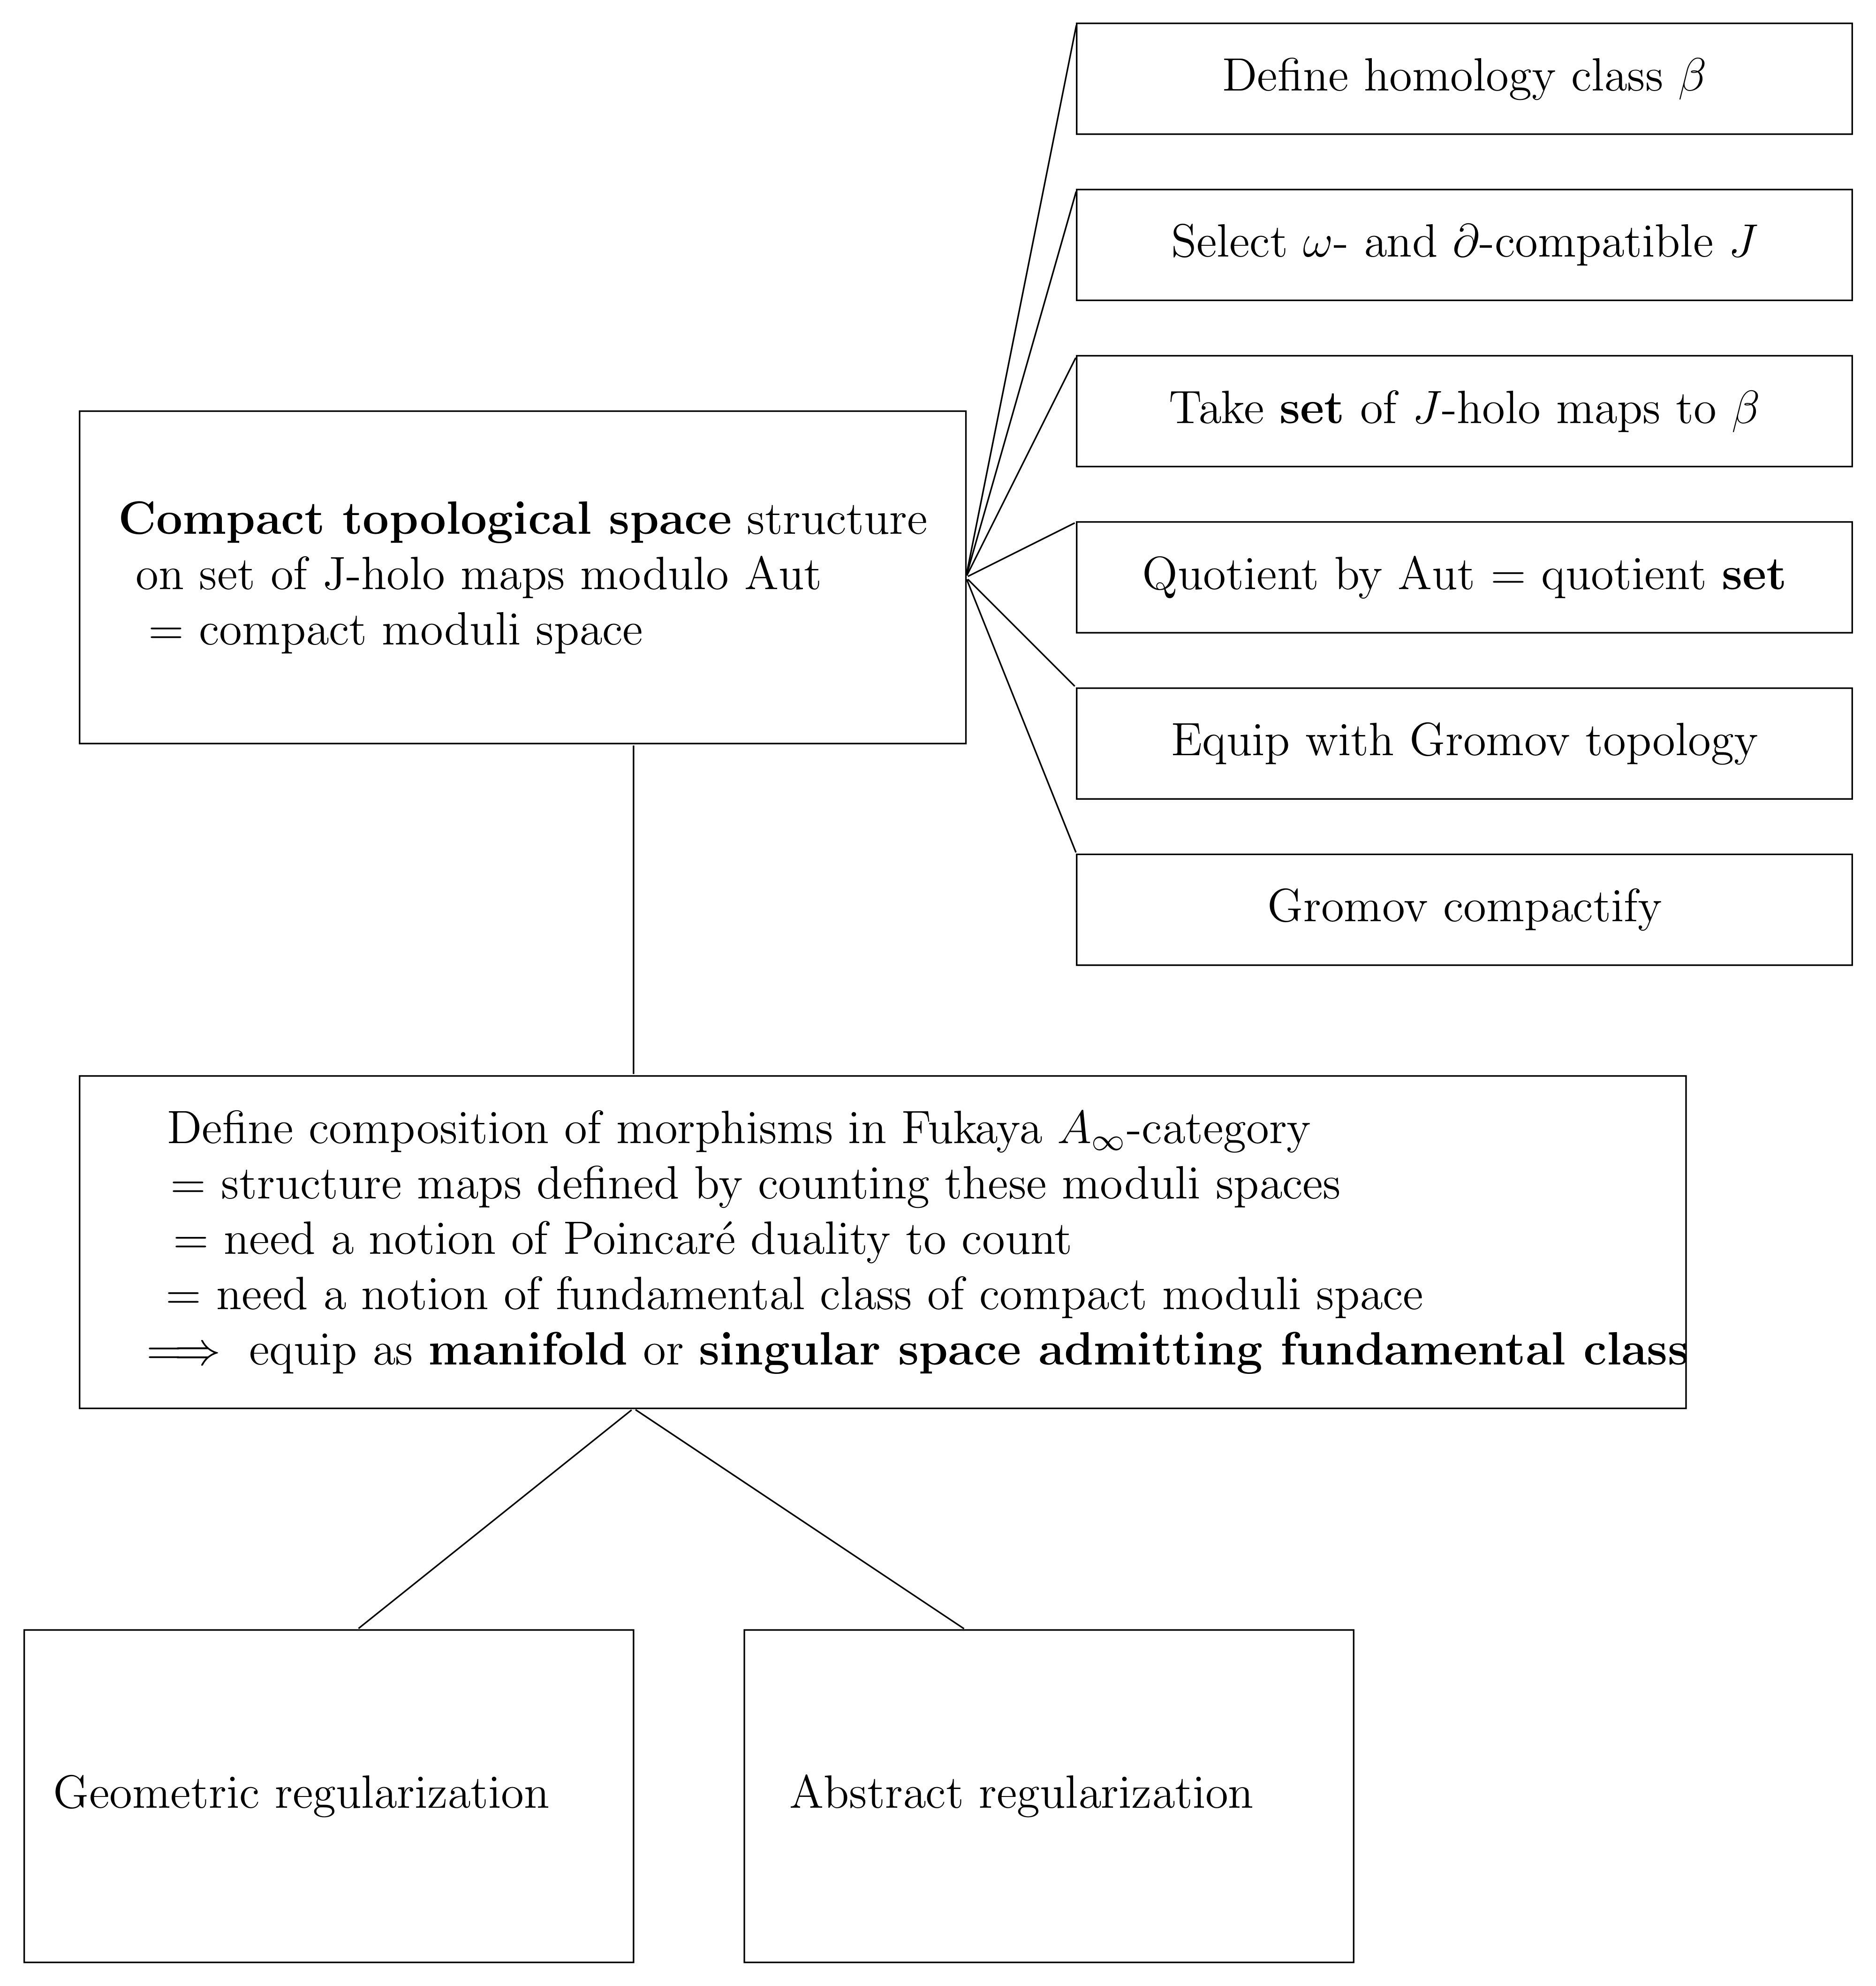
\includegraphics[width=0.84\textwidth]{figures/fig_4_3.png}
\caption{在深谷范畴中处理模空间的流程图（原书 p.96）}
\label{c7:fig-flow}
\end{figure}

% ===== 原书 p.97 =====

\begin{figure}[htbp]
\centering
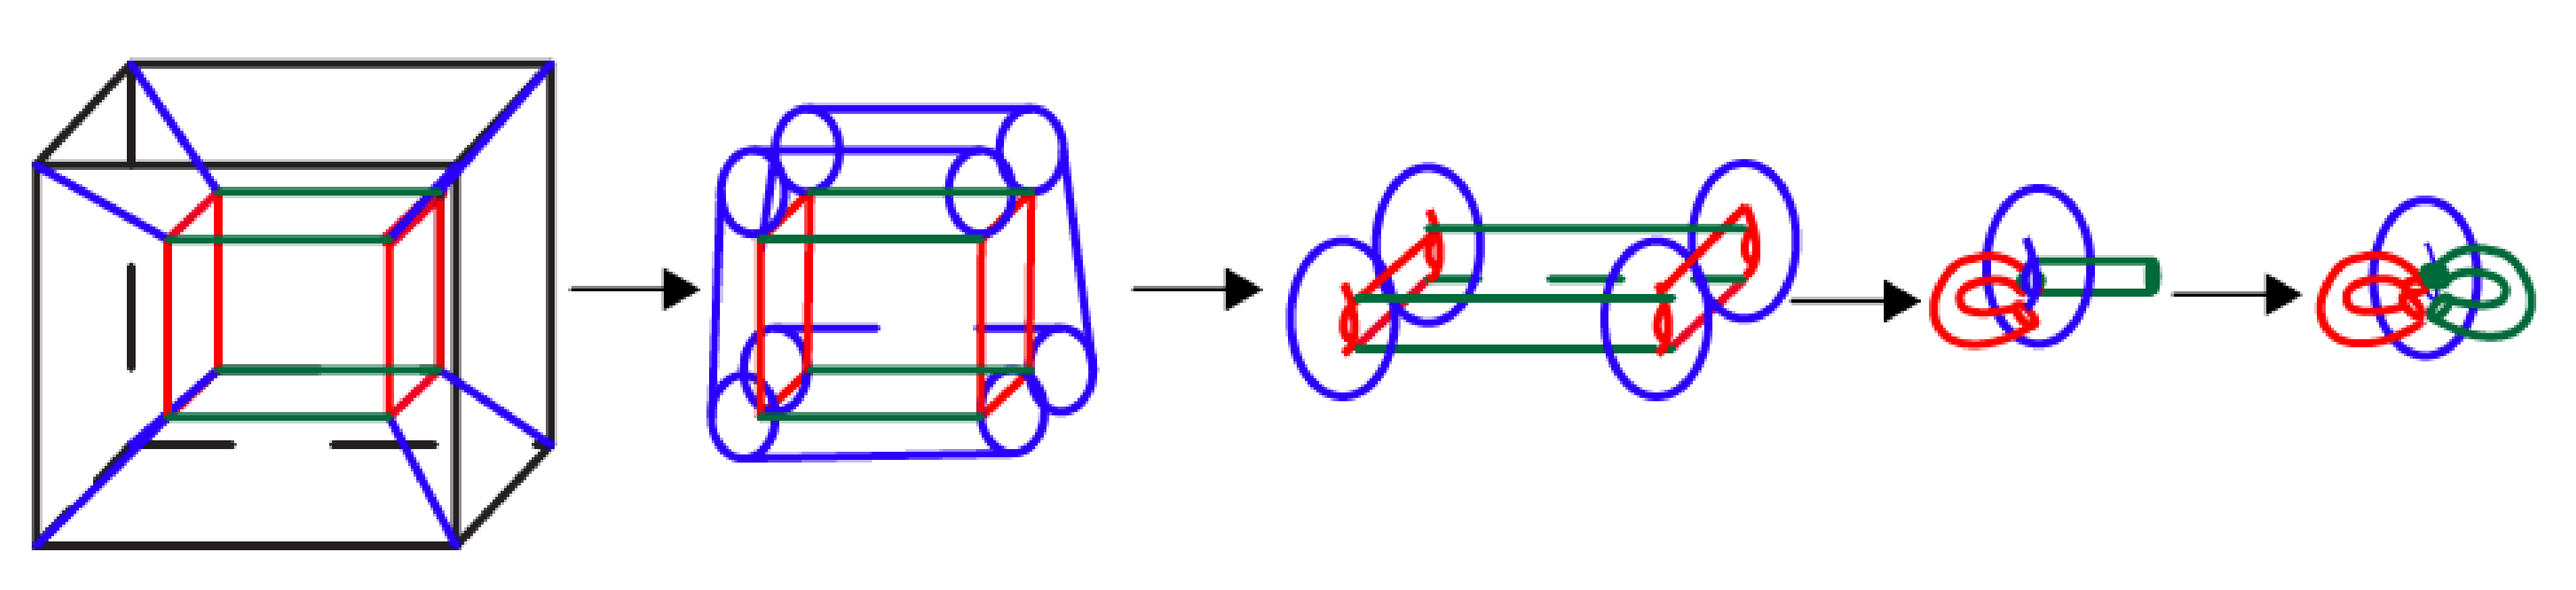
\includegraphics[width=0.95\textwidth]{figures/fig_4_4.png}
\caption{把 $T^4$ 看成 $4$-立方体的商所得胞腔复形的 $2$-骨架（原书 p.97）}
\label{c7:fig-2skeleton}
\end{figure}

\begin{remark}\label{c7:rem-spectral}
注意，我们把拓扑纤维化的谱序列直觉用到了纤维化 $v_0\colon Y\to\C$ 上。
它在代数几何意义下是纤维化，在代数拓扑意义下却不是，因为没有同伦提升性质。
例如取原点附近一个圆盘，由于奇点，把它提升上去有 $S^1$ 个选择。
也就是说，$T^4$ 与它的退化纤维 $\C\PP^2(3)/\Gamma_B$ 并不弱同伦等价。
若情形对得上，谱序列的第二页应是
\[
E^2_{p,q}=H_p(\C,H_q(T^4)).
\]

代数地看，带局部系统数的同调就是 $C_*(\tilde X)\otimes_\pi H_q(F)$。
这里 $\pi=\pi_1(\text{底空间})$ 作用在覆盖空间 $H_q(F_b)\mapsto b$ 上，取离散拓扑。
于是沿底空间中的单值性可以看见 $H_1(F_b)$ 的元素如何变化，这个变化给出 $\pi$ 的作用。
该链复形上的微分是 $\partial\otimes1$。
当万有覆盖 $\tilde X=\text{底空间}=\C$ 可缩时，$\pi_1$ 平凡，张量积就回到通常同调：$p>0$ 次为零，$p=0$ 次给出底空间的同调。
\end{remark}

\transnote{这里在解释「为什么不能直接用 Leray 谱序列算 $H_2(Y)$」：$v_0$ 只有代数几何的纤维化结构，没有同伦提升，故 $H_*(Y)$ 不能由 $H_*(\C,H_*(T^4))$ 的谱序列读出。作者的替代办法是先算中心纤维，再用 Mayer--Vietoris。}

\begin{remark}\label{c7:rem-toric}
另一种算法用 [CLS11] 的环簇理论。环簇 $X$ 内含一个稠密的 $(\C^*)^n$。
它是 $n$ 个柱面，可缩到 $n$ 个圆上，故 $\pi_1=\Z^n$。此外它满射到 $\pi_1(X)$，所以 $\pi_1(X)$ 总是 $\Z^3$ 的商。
本例在取商之前是 $\Z^4$：多面体中心给一个 $\PP^1$，三次爆破再给三个。
取商之后，香蕉流形中的三个 $\C\PP^1$ 加起来等于一个矩映射纤维与一个被捏的 $T^3$；特别地，第四个生成元是前三个之和。

令 $Z:=\widehat{\C\PP^2(3)}/\!\sim$，它的多面体由六边形的无限铺砌给出，正是 $\tilde Y$ 的中心纤维。
它是万有覆盖，理由是由环簇理论 $\pi_1(Z)=0$。
于是 Hurewicz 定理给出 $\pi_2(Z)=H_2(Z)$，进而 $\pi_2(\C\PP^2(3)/\!\sim)=\pi_2(Z)$。
因此要算 $H_2(\C\PP^2(3)/\!\sim)$，也可改用下面的 Mayer--Vietoris。

在六边形图中挖去一个开集，它会收缩到边界上。这样得到两个开集；在矩映射图像里，它们是一个圆盘与其补集，交于一个 $S^1$。

令 $B:=D^2\times T^2$ 对应矩多面体中的圆盘。令 $\tilde A$ 为其补集，是一圈 $6$ 个 $\C\PP^1$；再令 $A:=\tilde A/\Gamma_B$ 为香蕉流形。于是
\end{remark}

% ===== 原书 p.98 =====

\[
\begin{aligned}
0=H_3(\tilde A)\oplus H_3(B)&\longrightarrow H_3(Z)=0\\
&\longrightarrow H_2(\tilde A\cap B)=\Z^3
  \xrightarrow{\ (*)\ } H_2(\tilde A)\oplus H_2(B)=\Z^6\oplus\Z
  \longrightarrow H_2(Z)\longrightarrow 0\\
H_1(\tilde A\cap B)=\Z^3&\xrightarrow{\ \cong\ } H_1(\tilde A)\oplus H_1(B)=\Z\oplus\Z^2
  \longrightarrow H_1(Z)=0
\end{aligned}
\]
其中
\[
(*)=\begin{pmatrix}
1&0&0\\
0&1&0\\
-1&1&0\\
-1&0&0\\
0&-1&0\\
1&-1&0\\
0&0&1
\end{pmatrix},
\]
并且倒数第二个映射关于 $H_2(\tilde A\cap B)=H_2(S^1\times T^2)$ 的三个生成元是 $3\times3$ 恒等矩阵。
这三个生成元如下记：$b$ 记矩多面体中的 $S^1$，$T_1,T_2$ 记 $2$-环面纤维中的两个圈。
% [Tutor Note: 原文「倒数第二个映射」此处指 H_1 行的同构，却又说以 H_2(Ã∩B) 的生成元为基；H_1 与 H_2 的生成元一一对应，读者按后者理解即可。]

再对 $\C\PP^2(3)/\!\sim$ 取商，得到
\[
\begin{aligned}
0=H_3(A)\oplus H_3(B)&\longrightarrow H_3(\C\PP^2(3)/\!\sim)=0\\
&\longrightarrow H_2(A\cap B)=\Z^3
  \xrightarrow{\ (**)\ } H_2(A)\oplus H_2(B)=\Z^3\oplus\Z\\
&\longrightarrow H_2(\C\PP^2(3)/\!\sim)=\Z^4
  \longrightarrow \Z\cdot b\subset H_1(A\cap B)=\Z^3
\end{aligned}
\]
\[
\begin{pmatrix}
0&0&0\\
0&0&0\\
0&1&0\\
0&0&1
\end{pmatrix}
\longrightarrow H_1(A)\oplus H_1(B)=\Z^2\oplus\Z^2
\longrightarrow H_1(\C\PP^2(3)/\!\sim)=0,
\]
其中
\[
(**)=\begin{pmatrix}
0&0&0\\
0&0&0\\
0&0&0\\
0&0&1
\end{pmatrix}.
\]
% [Tutor Note: 原书此处自相矛盾：序列中的 4×3 矩阵第三行为 (0 1 0)，而页面下方「where (**)=」给出的矩阵第三行全零。译文照录两处，未作统一；请读者以序列中实际出现的矩阵为准，此点已登记疑点。]

所以最终我们看的是 $6$ 个 $\PP^1$ 射到三个粘起来的 $\PP^1$ 上的投影。同调仍是 $\Z^4$。

到这儿，我们知道了 $Y$ 中可以出现球泡像的同调类。还需要知道：边界落在给定拉格朗日上的圆盘的相对 $H_2$。
回忆背景一节中对映射与截面的讨论。下面定义本文要用的圆盘。
我们考虑的 $\pi_2(Y,L)$ 中的类覆盖底空间中 $0$ 附近的一个圆盘，并以一个点穿过中心纤维。
变动这个点，借助中心纤维的环簇几何可以枚举所有同调类，见 [CO06]。
这一点留到下文对某个 $J$ 计算圆盘计数时再说。这里只证明：给定 $H_2(Y,L)$ 中的同调类 $\beta$，相应模空间存在。

% ===== 原书 p.99 =====

\begin{definition}[类截面映射]\label{c7:def-section-like}
取原点附近的一个开集，记为 $U$。只考虑在 $U$ 外恒等于 $J_0$ 的近复结构。于是在 $U$ 外，圆盘就是截面。
由 Riemann 映射定理：若处处取 $J_0$，把该处的 $J_0$-全纯映射经也全纯的 $v_0$ 复合到底空间，这样的映射唯一。

为了得到足够好的正则性，需要允许 $J$ 在 $U$ 内部偏离 $J_0$。
具体地，下文所有拉格朗日都要求经过底空间中的点 $-1$。于是取 $U$ 为半径小于 $1$ 的圆盘，就可断定没有多重覆盖的圆盘，因为这类圆盘绕不过边界。
就取 $U$ 为以原点为心、半径 $1/2$ 的圆盘。

还能排除盘起泡与条带断裂：纤维中没有圆盘，因为环面中的线性拉格朗日相对 $\pi_2$ 为零，即它们不围出圆盘。
也不会有绕原点附近开集上圆盘边界的盘，因为它在 $-1$ 附近必须是一一的。
因此另一个盘或条带只能落在底空间圆周的真子集上方，而纤维化在那里可平凡化。
假设圆盘的边界落在 $U$ 外（但此时还需证明它对 Hamilton 同痕不变）；或者把盘在 $-1$ 附近的 $1$-$1$ 性质延拓到盘边界的其余部分。
两种做法都给出：由 $1$-$1$ 性质，这种盘的边界缩成一点；而环面中没有球，故该盘必为常值（或再次使用 $1$-$1$ 性质）。

若真出现多重覆盖，可以要求 $J$ 依赖 $z\in S$，即把 $J$ 换成 $J_z$。
[MS12] 为拉格朗日边界情形奠定了这一基础，[Aur14] 有具体描述，其中涉及条带上的一族 $\R$-参数 $J$。不过我们这里用不上。
\end{definition}

\transnote{取「半径 $<1$、圆心在原点」的 $U$，配合「拉格朗日过 $-1$」这条要求，是为了让任一多重覆盖盘都绕不到 $U$ 的边界上，从而被排除。若把 $U$ 取大，这条论证就断了。后文所有 $L_i$ 都过底空间中的 $-1$，原因也在此。}

\begin{corollary}\label{c7:cor-J-curve}
$J$-全纯曲线有一些与复曲线类似的性质。例如 Carleman 相似原理：一条近似满足 CR 方程的曲线，可经后复合一个映射，改为满足以 $J_0$ 写出的 CR 方程。这是辛流形 $\R^{2n}$ 的情形。
其余推论包括：唯一延拓，即两个 $J$-全纯映射若在开集上相等，或在一点处所有导数相等，则两者相等；原像中只有有限个点，临界点也只有有限个；简单曲线的单射点集是开稠密的。
\end{corollary}

曲线的像落在 $Y$ 的哪些同调类，前面已经讨论完。接下来证明正则 $J$ 存在。
有了它，就能构造一个 Fredholm 问题：Cauchy--Riemann 算子 $\bar\partial_J$ 作为 Banach 丛的截面切出模空间，再由隐函数定理得知零点的原像是流形。
这样就能给模空间安上光滑结构。

% ===== 原书 p.100 =====

\begin{example}\label{c7:ex-banach-analogy}
这是无穷维 Banach 空间中的一个类比。先看有限维的例子：$f\colon\R^3\to\R$，$f(x,y,z)=x^2+y^2+z^2$，在 $(x,y,z)\neq0$ 处正则，因为
\[
\de f|_{(x,y,z)}=(2x,2y,2z)^{\mathsf T}
\]
满射。于是 $f$ 是正则函数，$1$ 的原像是光滑流形（球面）。
在 Banach 丛的设定中，「正则」不仅要求满射，还要求右逆存在。
\end{example}

区别在于这里的微分算子以函数为输入，于是进入无穷维 Banach 空间的世界。
下面的理论沿用 [MS12, 第 3--10 章] 的论证，但针对带边曲线；[Sei08] 也有讨论。
[Weh13] 用几何正则化理论处理 Gromov 非挤压定理，示范了如何证明随 $J_t$ 变化的模空间族是 $1$ 维的（Fredholm）、是流形（横截/正则）、是紧的（Gromov 紧性），且有边界。
抽象正则化理论的好参考是 [Weh14]。

下面证明正则 $J$ 存在。

\begin{lemma}[几何正则化]\label{c7:lem-geometric-reg}
存在稠密子集 $\cJ^1_{\mathrm{reg}}\subset\cJ(Y,\omega)$，由在 $U$ 外恒为 $J_0$ 的 $\omega$-相容近复结构 $J$ 组成，使得对一切 $J$-全纯映射
\[
u\colon(D,\partial D)\to(Y,L|_\gamma),
\]
线性化 $\bar\partial$ 算子 $D_u$ 满射。这里的拉格朗日边界条件由「在底空间中从 $-1$ 出发绕 U 形平行移动纤维拉格朗日」给出。
\end{lemma}

\begin{remark}\label{c7:rem-superscr}
上标 $1$ 是为了后文：还要更小一些的 $\cJ^2_{\mathrm{reg}}$ 与 $\cJ^3_{\mathrm{reg}}$，分别对「盘接盘」「盘接球」正则，边界条件类似，标号取 $2$、$3$。
它们不仅要求线性化算子满射，还要求交点处的取值行为相容。
\end{remark}

\begin{proof}[{略证，改写自 [MS12] 第 2 版第 55 页编号 3.1.6(ii) 那条定理的证明}]
我们给一张路线图，把 McDuff--Salamon 的做法改写到带拉格朗日边界条件的情形。
相关背景也取自 [Weh14, 第 9 讲]；细节在 2017 年 9 月 8 日的 Denis 讨论班上讲过。
[MS12] 的定理 C.1.10 证明：带边界情形确有 Fredholm 问题。

\textbf{引言。}「正则化」指扰动 $\bar\partial_J$ 算子，使它等变横截于某个 Fredholm 丛的零截面；该丛可造得让这个算子成为其截面。
「几何正则化」指扰动来自对近复结构 $J$ 的扰动，因而具有几何来源。也就是说，$J'$ 变动时 $\bar\partial_J$ 的扰动是 $\bar\partial_{J'}-\bar\partial_J$。
在这种设定下，等变性自动成立，下文会说明。
注意后文计算要用非正则的 $J$；那时改用「抽象正则化」，即加抽象扰动 $\nu$。
$\nu$ 仍是同一 Fredholm 丛的截面，但不必是 $\bar\partial_{J'}-\bar\partial_J$ 的形式。
\end{proof}

\transnote{「几何正则化」与「抽象正则化」的区别是本节的主线：前者扰动 $J$ 本身，后者在 Fredholm 丛上加抽象截面 $\nu$。前者能做是因为 $J$ 的空间足够大且在边界附近已固定；后者在计算时不得不用，因为圆盘计数只需要 $J$ 的拓扑信息，而不需要它正则。}

% ===== 原书 p.101 =====

为证明「映到沿 U 形曲线平行移动所得纤维拉格朗日」的圆盘存在正则 $J$，我们证明这类 $J$ 在
\[
\cJ^\ell_\omega(Y,U):=\{J\in\Gamma(TY)\mid J^2=-1,\ J|_{Y\setminus U}\equiv J_0,\ J\in C^\ell\}
\]
中稠密。
在 [Sei08] 中它记作 $\cJ^\ell_F$，其中 $F$ 指「平行移动纤维拉格朗日」所得的拉格朗日边界条件，他称之为运动边界条件（moving boundary condition）。
带边界情形需要的正是这个 $J$ 集，参看 [MS12, Remark 3.2.3]。

先定义由变 $J$ 编码的「全体 $W^{k,p}$ 映射 $u$ 与几何扰动」之集：
\[
\cM_J:=\{(u,J)\mid J\in\cJ^\ell_\omega(Y,U),\ W^{k,p}\ni u\colon(D,\partial D)\to(Y,L)\}.
\]

$k$ 充分大时 $W^{k,p}\subset C^\ell$。再由椭圆自举可知 $J$-全纯映射 $u$ 属于 $C^\ell$。
这个模空间称为「万有的」，因为允许 $J$ 变动。
用 $W^{k,p}$ 是因为它完备，即 Banach 空间；在函数空间的无穷维设定里调用 Sard--Smale 与椭圆正则正需要这一点。
特别地，我们希望 $\cM_J$ 是 $C^{\ell-1}$ 的可分 Banach 流形。
然后对投影 $(u,J)\mapsto J$ 用 Sard--Smale，就得到圆盘的正则 $J$ 构成稠密集。

\textbf{Banach 丛的搭建。}
我们要把 $\cM_J\subset\cB^{k,p}\times\cJ^\ell_\omega(Y,U)\ni(u,J)\mapsto J$ 看成某个 Banach 丛的 Fredholm 截面，以便用 Sard--Smale 得到稠密的正则值集。
Fredholm 是满射的推广。在无穷维设定中还要求右逆存在；最近那篇 polyfold 文章里就有右逆不存在、且仅此不够的例子。
随后隐函数定理给出：该截面的零点切出的 $(u,J)$ 之集是底空间的 Banach 子流形，而不只是子集。
注意零点集正是使 $u$ 为 $J$-全纯的那些 $(u,J)$。

$\cB^{k,p}\ni u$ 上的 Banach 流形结构：在任意映射 $u$ 附近构造局部 Banach 图。
局部模型是 $T\Gamma(u^*TY,u^*TL)\ni\xi$，映射为 $u\mapsto\exp_u\xi$。
这是良定义的：总存在度量使一个拉格朗日全测地 [MS12, Lemma 4.3.4]；也就是说，从某个度量看，一个拉格朗日（或两个）是全测地的。
所考虑的点处至多有两个拉格朗日相交，所以够用。
带拉格朗日边界条件时，正需要全测地性来保证这给出图：给定 $\partial D$ 上一点，沿该点处放置的向量 $\xi$ 走，结果仍切于 $L$，于是测地线留在 $L$ 中。

$\cJ^\ell_\omega(Y,U)\ni J$ 上的 Banach 流形结构（它是所造 Banach 丛底空间的第二个因子，参看 [MS12, §3.2]）：同样用指数映射得到 $\dot J$。
$J$ 的三个条件线性化：1）$J|_{Y\setminus U}\equiv J_0$ 给出 $\dot J|_{Y\setminus U}\equiv0$，这是拉格朗日边界情形特有的；2）$J^2=-1$ 给出 $\dot JJ+J\dot J=0$；3）$\omega(\cdot,J\cdot)>0$ 且对称这一条也线性化。
图由 $J\mapsto J\exp(-\dot JJ)$ 构造。参看 [Sei08]。
丛的纤维不带边界条件，因为它由 $(du)^{0,1}=\frac12(du+J\circ du\circ j)$ 的落点空间给出，与边界无关。
至于切于边界的方向会发生什么，则不得而知，因为 $J$ 与 $j$ 可能把它们拧来拧去。

% ===== 原书 p.102 =====

下面说明如何在底空间的开集上搭起 Banach 丛的结构。这部分照抄 [MS12] 的做法，因为纤维上没有边界条件。
在 $\cB^{k,p}\times\cJ^\ell_\omega(Y,U)$ 的第一个因子上，用指数映射在邻域 $\cN(u)$ 上平凡化丛；在第二个因子上，用平行移动在邻域 $\cN(J)$ 上平凡化。
两者合起来把丛在底空间的一个邻域上平凡化；这些平凡化复合得到的过渡映射满足 Banach 丛的条件，见 [MS12] 与 [Sei08]。

\textbf{Fredholm 问题。}
Fredholm 问题就是 Banach 丛的 Fredholm 截面。
所谓 Fredholm 截面，指线性化为 Fredholm 算子的截面：$\dim\Ker-\dim\Coker$ 有限（例如到纤维切空间的投影满射），且像闭。
更一般地，它把模空间（主体部分，以及作为纤维积出现的 Gromov 紧化成分）搭成若干 Fredholm 截面的零点集。

我们断言截面 $(u,J)\mapsto\bar\partial_J(u)$ 是 Fredholm 的。
要取 $\bar\partial$ 算子在映射 $u$ 处的线性化，须看 $u$ 沿切向量 $\xi$ 作无穷小变动时会发生什么。
也就是把 $\bar\partial$ 算子放在一族中求导，再取零处的导数，见 [MS12, Proposition 3.1.1]。
同理，$J$ 沿切向量 $\dot J$ 作无穷小变动。
\[
\cF_u\colon W^{k,p}(S,u^*TY)\to W^{k-1,p}(S,\Lambda^{1,0}\otimes_j u^*TY).
\]

$D_u$ 的定义如下：对 $u$ 的指数邻域中附近的 $u'$，取 $D_{u'}\bar\partial_J$，把它沿平行移动送回 $u$ 处图的原点，作用 $\bar\partial_J$，再沿平行移动推回纤维上。
线性化算子 $D_u\xi$ 就是这一操作在 $0$ 处的导数。由上面全测地的条件，这是良定义的。
以上只变 $u$。若同时变 $J$，得到 [Weh14, 第 9 讲]：
\[
D_u\xi+\frac12\dot J\,\de u\,j .
\]

特别地，它满射且有右逆，从而是 Fredholm 的。理由如下。
反设像不稠密，取像的正交补中一个非零线性泛函 $\eta$。
令 $\dot J=0$，可见 $\eta$ 也正交于 $\mathrm{im}(D_u)$。于是它对一切 $\dot J$ 都正交于 $\dot J\,\de u\,j$。
但用鼓包函数，由 $\eta\neq0$ 可构造扰动 $\dot J$，使 $\eta$ 作用在其上的积分非零，矛盾。见 [MS12, 第 65 页]。

在拉格朗日边界情形中这个构造仍可行：所构造的 $\dot J$ 支在某个「某处单射」点附近的小邻域内，因此在边界附近为零，正合要求。
某处单射点稠密，故可在 $\eta$ 非零的给定点附近找到一个；特别地，这类点有邻域。
用鼓包函数构造 $\dot J$，使 $\int_D\eta(\dot J\,\de u\,j)>0$。这推出矛盾。

% ===== 原书 p.103 =====

于是 $\eta$ 在单射点的开集上为零，由唯一延拓 [MS12, Theorem 2.3.2] 恒为零。
这又与 $\eta\neq0$ 矛盾。故原假设「像不稠密」不成立。
像稠密；又因它闭，故满射且有右逆。

\textbf{Sard--Smale 与反函数定理。}
有了 Fredholm 问题，就可以用 [MS12, 附录 A：Fredholm 理论] 中关于 Banach 空间的结果。
特别地，我们满足 [MS12, Theorem A.5.1（Sard--Smale 定理）] 的假设，而该定理依赖无穷维反函数定理 [MS12, Theorem A.3.1（反函数定理）]。
Sard--Smale 的结论是：正则 $J$ 之集在全体 $J$ 中稠密，正是我们的目标。于是正则 $J$ 存在。

\begin{remark}[记号]\label{c7:rem-notation-Jdot}
注意：记号 $\dot J$ 并不意味着只能在某个方向上变 $J$，通常点记号有此含义。
这里只是把 $\dot J$ 当作「复结构空间切向量」的象征性写法。
文献中这个空间常记作 $Y$，但本文 $Y$ 指 A 侧的流形。
\end{remark}

\begin{lemma}\label{c7:lem-param-discs}
对 $J\in\cJ^1_{\mathrm{reg}}(Y,\partial Y)$，参数化的 $J$-全纯圆盘 $u\colon(D,\partial D)\to(Y,L|_\gamma)$ 之集是有限维流形。
\end{lemma}

\begin{proof}[{取自 [MS12, Theorem 3.1.6(i)] 的证明}]
图由
\[
\cF_u\colon W^{k,p}(S,u^*TY)\to W^{k-1,p}(S,\Lambda^{1,0}\otimes_j u^*TY),
\qquad
\xi\mapsto\exp_u\xi
\]
给出：把 $\cF_u^{-1}(0)$ 中 $u$ 附近的开集微分同胚到 Banach 空间中 $0$ 附近的相应开集。
$J$ 的正则性给出 $\de\cF_u(0)=D_u$ 满射。
隐函数定理 [MS12, Theorem A.3.3] 说明，适当缩小开集后这些就是光滑流形的图。
这与 $k,l$ 无关，因为由椭圆正则 [MS12, Proposition 3.1.10]，$J$-全纯映射 $u$ 是光滑的。
注意 [MS12, 附录 B（椭圆正则）] 已就全实边界条件（例如这里的拉格朗日边界条件）备好所需背景。
此处不重写证明，只定义该节用到的术语，另见 [Weh13, 第 4--6 讲]。
\end{proof}

\begin{itemize}[leftmargin=1.6em,itemsep=0.2em]
\item $C^k_0$：$k$ 次连续可微，且到该阶为止的导数在无穷远处趋于零。
\item 检验函数的 Schwartz 空间 $\zeta$：满足 $f\cdot(\sqrt{1+|x|^2})^k\in C_0$ 的 $f$。
      它对卷积封闭，且结合。缓增分布（tempered distributions）$\zeta'$ 指其对偶空间。
      特别地，$\zeta\hookrightarrow\zeta'$，嵌入由连续稠密单射 $f\mapsto\int_{\R^n}f\cdot(\cdot)\,\de^nx$ 给出。
\item 说一个等式「弱意义下成立」，意思是「对所有缓增分布积分后成立」。
\end{itemize}

% ===== 原书 p.104 =====

\begin{itemize}[leftmargin=1.6em,itemsep=0.2em]
\item Fourier 变换在 Schwartz 空间上是连续映射，并把卷积变成乘法。
\item Sobolev 空间 $W^{s,2}$：满足 $F.T.(f)\cdot(\sqrt{1+|x|^2})^k\in L^2$ 的 $\hat f\in\zeta'$。
      $W^{k,p}$：到 $k$ 阶的导数弱意义下属于 $L^p$。
      特别地，$k\gg l$ 时有紧支的 Sobolev 嵌入 $W^{k,p}\subset C^l$。
\item 函数 $u$ 的支集是「$u=0$ 处」在弱意义下的补集。
      分布 $u$ 的奇支集，指弱意义下挖掉那些具有局部紧光滑性的 $u\in\zeta$ 之后剩下的部分。
% [Tutor Note: 原文这句「The singular support of a distribution means we remove, in a weak sense, u ∈ ζ with no local compact smoothness」表述含混，字面如此照译，请读者按标准定义（奇支集 = 光滑性失效处的闭集）理解。]
\item 椭圆正则：$p(D)u$ 光滑，当且仅当 $p(D)$ 的奇支集为空，当且仅当 $u$ 光滑。
      特别地，$\bar\partial u=0$ 推出 $u$ 光滑。
      当 $p>2$ 时，导数的 $L^p$ 界给出紧模空间。
      $p=2$（即 $L^2$ 范数）时这一点失效，于是可能起泡，泡不在模空间里。
      要紧化，就商掉区域的自同构群，并确定可能起什么泡。
      随后需要把泡现象粘回主体，才能得到紧流形。这些 Gromov 紧性现象见 [Weh13, 第 7--9 讲]。
\end{itemize}

\begin{remark}\label{c7:rem-nonregular-J}
即使 $J$ 非正则，仍可用上面的办法，借助 [MS12, Theorem C.1.10（Riemann--Roch）] 构造 Fredholm 问题；该定理已在拉格朗日边界情形下证明。
但光滑结构从何而来是另一回事，因为 $J$ 不正则。抽象扰动可能正是在这里派上用场。
\end{remark}

\begin{example}[区域的模空间]\label{c7:ex-dm-space}
Deligne--Mumford 空间：把稳定曲线（亏格 $g$、$k$ 个标记点）映到一点，再对重参数化取商。
要紧化并纳入所有可能的余维 $1$ 构型，即稳定曲线的极限，需考虑合适的对偶图。参看 [Sei08, §9] 与 Liu 关于对偶图的文献。

一棵树记录如何粘接：内部边配一个粘接长度，两端半无限边给出最终粘好的圆盘的标记点。
想法是：我们有一族圆盘，由底空间中可能的循环构型参数化；每条内部边还配一个粘接参数。
内部边越多，底空间维数越高，因为泡占掉的余维越多。

再把所有 $d$ 叶树添进去，就得到该族底空间的紧化。
只要 $\overline\cR^{d+1}$ 上第二可数与 Hausdorff 两条成立，就能定义连续性、拓扑与光滑性。
按 FOOO 的说法，这些性质是从 Deligne--Mumford 空间 $\overline{\cM}_{0,d+1}$ 的实轨迹子集继承来的，因为粘接参数是实的。
多边形正则性与层论解释另见 [Sei08, §13]。
\end{example}

% ===== 原书 p.105 =====

\begin{claim}\label{c7:claim-expected-dim}
给定 Fredholm 截面，可以算出参数化曲线流形的预期维数；未参数化曲线的模空间维数比它少三。此外还有诱导定向。
\end{claim}

Morse 理论中的类比：有了 Morse--Smale 数据，数特征值就知道模空间的维数。
$x^-$ 的不稳定流形与 $x^+$ 的稳定流形横截相交；投影映射从不稳定流形打到稳定流形的正交补。
Fredholm 截面的指标是 Hessian 的谱流（Morse 情形则是数 Hessian 矩阵的特征值）。
谱流来自 $(J_0\partial_t+S_s)_{s\in\R}$；$D_u$ 等于它加上 $\partial_s$ 再加一个紧扰动。

\begin{claim}\label{c7:claim-aut-action}
$\Aut$ 光滑地作用在参数化曲线流形上，故模空间 $\widehat\cM/\Aut$ 是光滑流形。
\end{claim}

\begin{claim}\label{c7:claim-gluing}
用粘接可以给紧化后的模空间安上光滑结构。所粘接的构型正是 Gromov 紧性中出现的那些。
于是得到光滑紧 $0$ 维流形的结构，可以数了。
\end{claim}

\begin{proof}[{略证，参看 [MS12] 与 [Weh13]}]
Gromov 紧性由若干结果推出，例如等周不等式
\[
|a(\gamma)|\le C|\mathrm{length}(\gamma)|^2,
\]
可去奇点定理与能量衰减。
这些结果告诉我们圆盘可能的极限构型有哪些：边界点处的盘泡、球泡，或条带断裂。
\end{proof}

\textbf{作为拓扑空间紧化。}
然后说明任一盘泡、球泡或条带断裂都是某列 $J$-全纯曲线的极限。
做法是先预粘接：把这些映射拼起来，拼出的可能不是 $J$-全纯的；再用 Newton 迭代把它变成 $J$-全纯映射。

结论是：未参数化模空间的边界，即 $\widehat\cM/\Aut\setminus\cM/\Aut$，是若干模空间在交点处取纤维积的结果。
例如会出现一个成分，由盘的模空间与球的模空间在公共交点上取纤维积，用以计入球起泡。
% [Tutor Note: 原文文字层两处均写作带帽的 M/Aut；页图上第一项的 M 除 hat 外还多一条上划线，第二项只有 hat，原书此处上划线疑为排版残留。译文第一项取 \widehat\cM、第二项取 \cM（据上下文应为未紧化部分，此时两项不同，差集非空）。]

\textbf{作为光滑流形紧化：极限构型的正则 $J$ 存在。}
要完成「模空间是紧光滑 $0$ 维流形」的略证，还需为这些额外的纤维积构型证明正则 $J$ 存在。
如上所述，靠 $Y$ 的几何可以排除盘起泡与条带断裂，于是只需考虑中心纤维中的球起泡。
盘与球相接处多出一个点，意味着需要「额外数据」的概念来记账这些特殊点。

\begin{definition}[稳定映射的模空间]\label{c7:def-stable-maps}
稳定映射由一棵树给出，树的每个顶点 $\alpha$ 是一个球泡，只有原本的主球例外。
「稳定」指的是没有非平凡自同构；特别地，固定三个点后就没有非平凡自同构。
伪闭链（pseudocycle）指模空间边界的像在全空间中余维至少为 $2$。
虚拟维数等于 Maslov 指标减去稳定树的边数的两倍。也就是说，每多一个起泡的球，维数降 $2$。
半正（semipositive）指对一般的 $J$，不存在负 Chern 数的 $J$-全纯球；本文正是这种情形，因为是 Calabi--Yau。
所得模空间的定义是：取一族映射，对重参数化取商，再紧化。
\end{definition}

% ===== 原书 p.106 =====

\begin{lemma}[有界能量曲线收敛到树的 Bolzano--Weierstrass 类比]\label{c7:lem-bolzano}
稳定映射的模空间具有 Gromov 收敛性。
\end{lemma}

参看 [MS12, 第 5 章]。记 u.c.s.\ 为「在紧子集上一致收敛」。
若固定同调类中各曲线的导数在某个 $p>2$ 的 $W^{1,p}$ 中有界，则得到 Bolzano--Weierstrass 型结论：任何序列都有收敛子列。
但在临界情形 $p=2$（本文即是），极限可能不在原来的曲线类中。
Gromov 收敛到稳定映射的意思是：对树的每个顶点 $\alpha$，有一族重参数化 $\phi^\nu_\alpha$；标记点保持不动，至少在极限中不动。

我们用下面的术语引入「纳入曲线极限」所需的物件，也就是得到紧模空间。
有限能量仍可能起泡，因为能量在缩放不变：自变量反比缩放，微分形式则按比例缩放。
不过导数可以爆破，例如 $\C\PP^1\to\C\PP^2$，$[x:y]\mapsto[x^2:\eps y^2:xy]$。
它参数化的是 $\C\PP^2$ 中由 $ab=\eps c^2$ 给出的全纯曲线。
$\eps\to0$ 时只得到曲线 $[x:0:y]$。但像的极限其实是两个球 $ab=0$，而不只是 $b=0$，因为 $\C\PP^2$ 中做了重整化：看 $ab=\eps c^2$，令 $\eps\to0$ 得 $ab=0$。

去掉起泡点后，曲线列 u.c.s.\ 收敛到主成分。
要找其余泡成分，取由 $z/R_n$（$R_n\to\infty$）定义的新曲线，并添上一列趋于泡点的点。
主体与各泡的能量之和应等于原能量；极限中能量不变。

$e_i$ 记 $\frac12|\de u_i|^2$。为得到到主成分的 $C^\infty_{\mathrm{loc}}$ 收敛，我们在能量上用 Bolzano--Weierstrass 定理。
主成分在 $S$ 上完全有定义（尽管我们挖掉了泡点），理由是伪全纯映射的可去奇点性质。

\begin{lemma}[稳定映射的 Gromov 紧性，参看 [MS12, Equation (5.1.5)]]\label{c7:lem-gromov-compact}
未参数化曲线（即等价类）模空间的紧化，是「各种可能的泡树对应的未参数化曲线」之并。
\end{lemma}

% ===== 原书 p.107 =====

\begin{proof}[{略证}]
理由是这些就是可能的极限构型。式 (5.1.5) 在特殊点情形给该集合配上拓扑，随后讨论粘接与该设定下的 Fredholm 问题。
\end{proof}

特别地，我们需要粘接，并讨论「一个盘加一个球」的 Fredholm 问题。
然后证明：某处单射的盘与简单球之并的模空间是负维数的流形，即空集，可以排除。

\begin{lemma}[排除本文设定中的起泡]\label{c7:lem-excluding-bubbling}
存在稠密子集 $\cJ^2_{\mathrm{reg}}(Y,\partial Y;D\cup\PP^1)$，其中的 $J$ 对「中心纤维中的简单球与某处单射的盘之并」的模空间正则；该盘是类截面的，故必为简单盘。
\end{lemma}

\begin{corollary}\label{c7:cor-no-bubbling}
上述正则 $J$ 对应的模空间维数为负，即空集。
特别地，任何经过开集 $U$ 的某处单射盘与任意「多重覆盖球与简单球」构型之并，其模空间都可排除。
\end{corollary}

\begin{proof}
Riemann--Roch 定理 [MS12, 附录] 给出：该正则 $J$ 切出的流形维数为负，具体是 $-2$。
Lazzarini 的结果 [Laz11] 说明任何盘都可分解为简单盘；他的另一篇 [Laz00] 证明任何 $J$-全纯盘都含一个简单 $J$-全纯盘。
于是若推论所述构型非空，则「简单盘与简单球之并」给出非常值映射——做法是经多重覆盖分解，取一个穿过该球的简单盘。
这与维数为负矛盾，故这样的非空模空间本就不存在。
\end{proof}

\begin{proof}[{引理 \ref{c7:lem-excluding-bubbling} 的证明}]
对每个成分（盘与球）分别有稠密的正则 $J$ 之集：盘的情形前面已述，球的情形见 [MS12, 第 3 章]。
要证的是：这两个稠密集之交中仍有稠密子集，且在 $0$ 上方盘球相交处行为良好。

\textbf{分别对球与盘的正则 $J$ 稠密集取交。}
考虑
\[
\cU\subset\cJ^2_{\mathrm{reg}}(Y,\partial Y;D\cup\PP^1)\times\cJ^1_{\mathrm{reg}}(Y,\partial Y),
\]
并要求 $u_D(D)\nsubseteq u_{\PP^1}(\PP^1)$；只有球的情形要求像不相等，与此相对。
我们有点态约束：球与盘在一点相接。因此需要赋值映射 $\cU\to Y\times Y$ 的横截性。

用 Sard--Smale 可以推出 $\cU$ 是流形；另需一项检查，涉及各成分上的零化子，如下。这取自 [MS12, 第 6 章]。
设 $L^q$ 形式 $\eta$ 在「盘球交点处取零」的 $W^{1,p}$ 测试向量 $\xi$ 上零化 $D_u\xi$。
无论把该交点看成球上的点（McDuff--Salamon 的做法）还是盘上的点（与 [MS12] 同一证明，只是几何约束更多、空间更小，需要测试的更少），$\eta$ 实际都有 $W^{k,p}$ 正则性。
回忆 [MS12] 的椭圆自举结论是对拉格朗日边界条件证明的。分部积分给出 $D^*\eta=0$。

% ===== 原书 p.108 =====

这是把 Stokes 定理与乘积法则用到 $\ip{\eta}{\xi}$ 上：$\eta$ 与 $\xi$ 在 $1$-形式上作赋值、在丛上作内积。
特别地，$\eta$ 与测试向量 $\xi$ 在边界处都切于拉格朗日，这保证相应的积分为零。

隐函数定理给叉积
\[
\cJ^2_{\mathrm{reg}}(Y,\partial Y;D\cup\PP^1)\times\cJ^1_{\mathrm{reg}}(Y,\partial Y)
\]
安上 Banach 子流形结构；此时再用赋值映射保证横截。
于是对角线的原像不只是子集，而是子流形，正是引理所要的稠密正则 $J$ 之集。
这些在 [MS12, §3.4] 的一系列引理中完成；由于附录中的定理都是对拉格朗日边界条件证的，这些引理适用。

\begin{itemize}[leftmargin=1.6em,itemsep=0.2em]
\item 要赋值映射横截。盘与球须在定义域中的 $0$ 处相交，因为 $v_0$ 的中心纤维正是 $H_2$ 非零之处。
      另外固定盘边界上一点，以消去非平凡自同构。
\item 要证赋值映射横截，只需构造支在小球中的 $\dot J$，每个成分一个球；每个球不与该成分之外的部分相交。
      因为前面看的是各成分模空间乘积中的 $\cU$（那个「半程步骤」），这样的开集找得到。
\item 这可行，因为：1）拉格朗日边界条件给出 $\dot J$ 在边界附近为零，故只支在内部小球上就是这种形式；2）各 $\dot J$ 零延拓后可以相加。
      要检查横截性，需线性化映射满射。于是在余空间 $(0_D,0_{\PP^1})$ 处取两个切向量，再在交点附近的两个小球上构造两个 $\dot J$，即得横截。
\item 要证这样的 $\dot J$ 存在，需要关于「在 $D_u$ 上为零的形式 $\eta$」的正则性与消失性结果。
      因为有了它，$D_u\xi+\frac12\dot J\,\de u\,j$ 就满射到 $W^{k-1,p}$ 空间，我们有足够自由度找到上面的向量。
      带边界条件时，附录中的引理与分部积分都成立：取伴随后边界项是 $\de\ip{\eta}{J\xi}_\omega$；边界上拉格朗日与 $\omega$-相容性一起使该项为零。故这一切在此设定下都行得通。
\end{itemize}

在万有空间中满足点态约束的子集上用 Sard--Smale，得到稠密的正则 $J$ 之集，使盘与球在其交点处的赋值映射横截。
引理 \ref{c7:lem-excluding-bubbling} 证毕。
\end{proof}

\textbf{极限构型构成光滑流形。}
极限构型的正则 $J$ 已有，下面证明 $\bar\partial_J$ 横截地切出
\[
\widehat\cM_D/\Aut\times_0\widehat\cM_{\PP^1}/\Aut,
\]
从而是流形。要得到流形结构，仍需 Banach 丛的一个 Fredholm 截面，且其线性化算子满射、有右逆。

% ===== 原书 p.109 =====

令 $\Sigma$ 为「圆盘在一个固定边界点处与球在原点相接」所得的黎曼面。
如上，给 $W^{k,p}(\Sigma,Y)$ 安 Banach 流形结构：用以切空间为模型的图；切空间是 Banach 流形。
也就是说，用指数映射描述「接近」给定映射 $u$ 的映射：给一点 $u$ 及该点处切方向 $\xi$，沿 $\xi$ 方向的测地线（即所需作用量最小的路径）走时间 $1$，得到新的 $W^{k,p}$ 映射 $\exp_u\xi$，它把 $u$ 处处沿 $\xi$ 方向略微推动。

我们要保持 $u_D\colon D\to Y$ 上的拉格朗日边界条件：若 $\xi$ 切于 $L$、$z\in\partial D$，则 $u_D(z)\in L$，并要求 $\partial D$ 上的 $\exp_{u_D}\xi$ 仍在 $L$ 中。
换言之，若沿切于 $L$ 的方向 $\xi$ 把 $u$ 推开，新映射的边界仍要落到指定的拉格朗日上。
换一种说法：测地线若起点在 $L$、初速切于 $L$，就应留在 $L$ 中。这正是全测地的定义。故 $L$ 必须全测地。
注意测地线与「作用量最小」只有在 $Y$ 上给定度量后才有意义。所以需要 $Y$ 上的一个度量，使涉及的所有拉格朗日都全测地。
使一个拉格朗日全测地的度量，其存在性由 Urs Frauenfelder 的学位论文证明，见 [MS12, Lemma 4.3.4]。
交点处至多有两个拉格朗日；使两者都全测地的度量，其存在性见 [Mil65, Lemma 6.8]。
Whitney Trick 讲义 [Fra10, Lemma 0.6, 第 11 讲] 有自足的陈述，证明续于 [Fra10, 第 12 讲]。

Banach 丛的纤维不必操心边界条件，参看 [Sei08, §(8h)]。

正则 $J$、以及从带点态约束的曲线的 $\bar\partial_J$ 零点集得到光滑流形这两件事，比之前只处理圆盘时多几项检查。
列举如下，依 [MS12, §3.4]。

\begin{itemize}[leftmargin=1.6em,itemsep=0.2em]
\item 局部构造一个 $\eta$，它落在 Banach 丛的纤维中。
\item 证明 $\eta$ 有 $W^{k,p}_{\mathrm{loc}}$ 正则性；上一步之所以局部地看，正为此。
\item 有了正则性，就可积分得到 $D^*_u\eta=0$。
\item 然后写出 $D^*_u\eta$，用 Carleman 相似原理：若 $\eta$ 在开集上为零，则它恒为零。
\item 由此可证某个空间的零化子为零；Hahn--Banach 于是给出稠密性，再结合 Fredholm 性质带来的闭性，
      得：含 $J^l$ 的线性化算子实际满射到 $W^{k-1,p}$。
\end{itemize}

% ===== 原书 p.110 =====

\begin{itemize}[leftmargin=1.6em,itemsep=0.2em]
\item 仍在单个成分（$\PP^1$ 或 $D$）上。满射性说明：可以找到 $\xi$，在指定点处指向指定方向，且切于模空间。
      先做前者，再用上一条改成后者。
\item 而且可在指定点附近的小邻域内做到。于是可以叠加作用于不同成分的向量。现在引入 $\PP^1\cup D$。
\item 由于（线性化的）赋值映射在向量上满射，万有模空间是流形，故正则 $J$ 稠密；于是取正则 $J$ 的模空间是流形。
\item 完毕：椭圆自举与隐函数定理在 [MS12] 附录中对拉格朗日边界条件已有覆盖。
\item 注：可用 $C^\infty_\eps$ 拓扑编码渐近行为，见 [Sei08, Remark 9.9]。
\end{itemize}

至此所有类型的起泡行为都排除了。所以模空间 $\widehat\cM/\Aut$ 已是紧流形，证明完毕。
现在可以取它们的 $0$ 维部分，用于下文深谷范畴的构造。

\begin{corollary}\label{c7:cor-general-disc}
上述结论对带任意多个拉格朗日、以及带条状端的 puncture 的盘都成立，理由如下：使两个拉格朗日都全测地的度量存在，见 [Mil65, Lemma 6.8]。
\end{corollary}

\transnote{原书 4.3.22 那条推论把前面「两个拉格朗日」的讨论推广到任意多个：每个交点至多涉及两个拉格朗日，逐个用 [Mil65] 的度量再把它们粘起来，就得到使所有涉及的拉格朗日都全测地的度量（粘法为译者补足，原文只说度量存在）。原文只用一句话带过，未展开粘法。}
